\documentclass{deliverablereport}

\deliverable{dissem}{ibook1}
\deliverydate{31/08/2018}
\duedate{31/08/2018 (M36)}
\author{Marcin Kostur, Jerzy Łuczka, Jan Aksamit, Jolanta Marzec}

\begin{document}
\maketitle

\tableofcontents
% \githubissuedescription

\TODO{What about dedicating this document to the memory of Jan Aksamit?}

\section{Introduction}

Interactive web pages have always been an attractive tool in
education. It has started in the age of Adobe-Flash technology, when a
lot of educational material was created. The advent of JavaScript has
led to significant improvements in that field: in the first place it
created a possibility to author the content using Open Source tools
and secondly it increased the portability of the created documents to
practically all devices equipped with a modern web browser.

The problem which was persistent in those solutions was the big gap
between the authoring process of interactive documents and their usage.
Usually the code behind an interactive examples was not very
educational and was not supposed to be edited by the student.

Then emerged the concept of interactive widgets in the notebook,
appearing first in Mathematica, then being popularized by the \Sage
notebook, and recently getting huge traction with the \Jupyter
notebook thanks to its wide audience. Interactive widgets, and in
particular the very simple to use \texttt{@interact} decorator,
delivered a versatile solution to this problem: they made it possible
to turn with little efforts a mere scientific calculation into a
visually appealing interactive application, all within the original
environment where the mathematical explorations took place.

\TODO{The above lays out nicely the context about the needs for
  teaching and the technology evolution. Now state very briefly:
  - what did you start from: what kind of material had been previously
    authored? using which technology?
  - what was achieved for this deliverable: in section ... we report
    on the writing of a book on XXX for audience YYY
  - some figures: how many pages? how many interactive figures? language? how
  many students are reading it? how many PM's were spent on the project...}

The source code of the interactive books is hosted on github within a
dedicated repository of the OpenDreamKit organization:
\url{https://github.com/OpenDreamKit/iODKbook2}.


\section{Interactive book technology}

We have used \Sphinx as main authoring tool: \Sphinx is originally a
documentation generator which is popular in the Python world where
it's used for the documentation of \Python itself, and many other
projects. More generally it can be used to author large structured
documents which are then exported to various formats, including HTML,
PDF, EPub, and now even Jupyter notebooks. \Sphinx contains a plugin
system enabling to taylor it for particular applications. We used
plugins for
\begin{itemize}
\item embedding \Sage code as live cells which can be edited, executed
  and interacted with (see Figure~\ref{fig:interact_sphinx}); under
  the hood the computations are run on a remote service thanks to the
  SageMathCell technology; an alternative would be to use Thebelab
  (see~\longdelivref{UI}{ipython-kernels});
  \TODO{NT: after the report, we should discuss this! I wrote a similar
    extension to use thebelab in Sphinx; see my class notes at
    \url{https://more-sagemath-tutorials.readthedocs.io/en/latest/agregation-option-calcul-formel/multiplications_rapides.html}.}
\item using conditional compilation of parts depending for example on
  whether the target medium is interactive of not\TODO{, or whether
    solutions should be included}\TODO{NT: I want this feature for my course!!!!}.
\item automatically including \Jupyter notebooks with embedded output;
\item producing high quality pdf via \LaTeX system.
\end{itemize}
\TODO{The first two??? were developed in house and distributed at ...???}

In the authoring process one can join interactive material in the form
of notebooks (based on sagenb or \Jupyter) that can be embedded in
full or in part into the \Sphinx book. In the HTML export, the
material is then rendered as live SageCellServer code that the user
can edit, execute, or interact with. It has to be stressed that not
only interactive widgets written with \texttt{@interact} are useful.
Practically all of the \TODO{XXX} exercises inside the book are
illustrated by such interactive material. It's our experience however
that such interactive material should not require or encourage the
reader to do anything but small edits to the provided code; indeed
such edits are volatile by essence; they take place anonymously in the
browser with no storage behind the scene.

\begin{figure}
\centerline{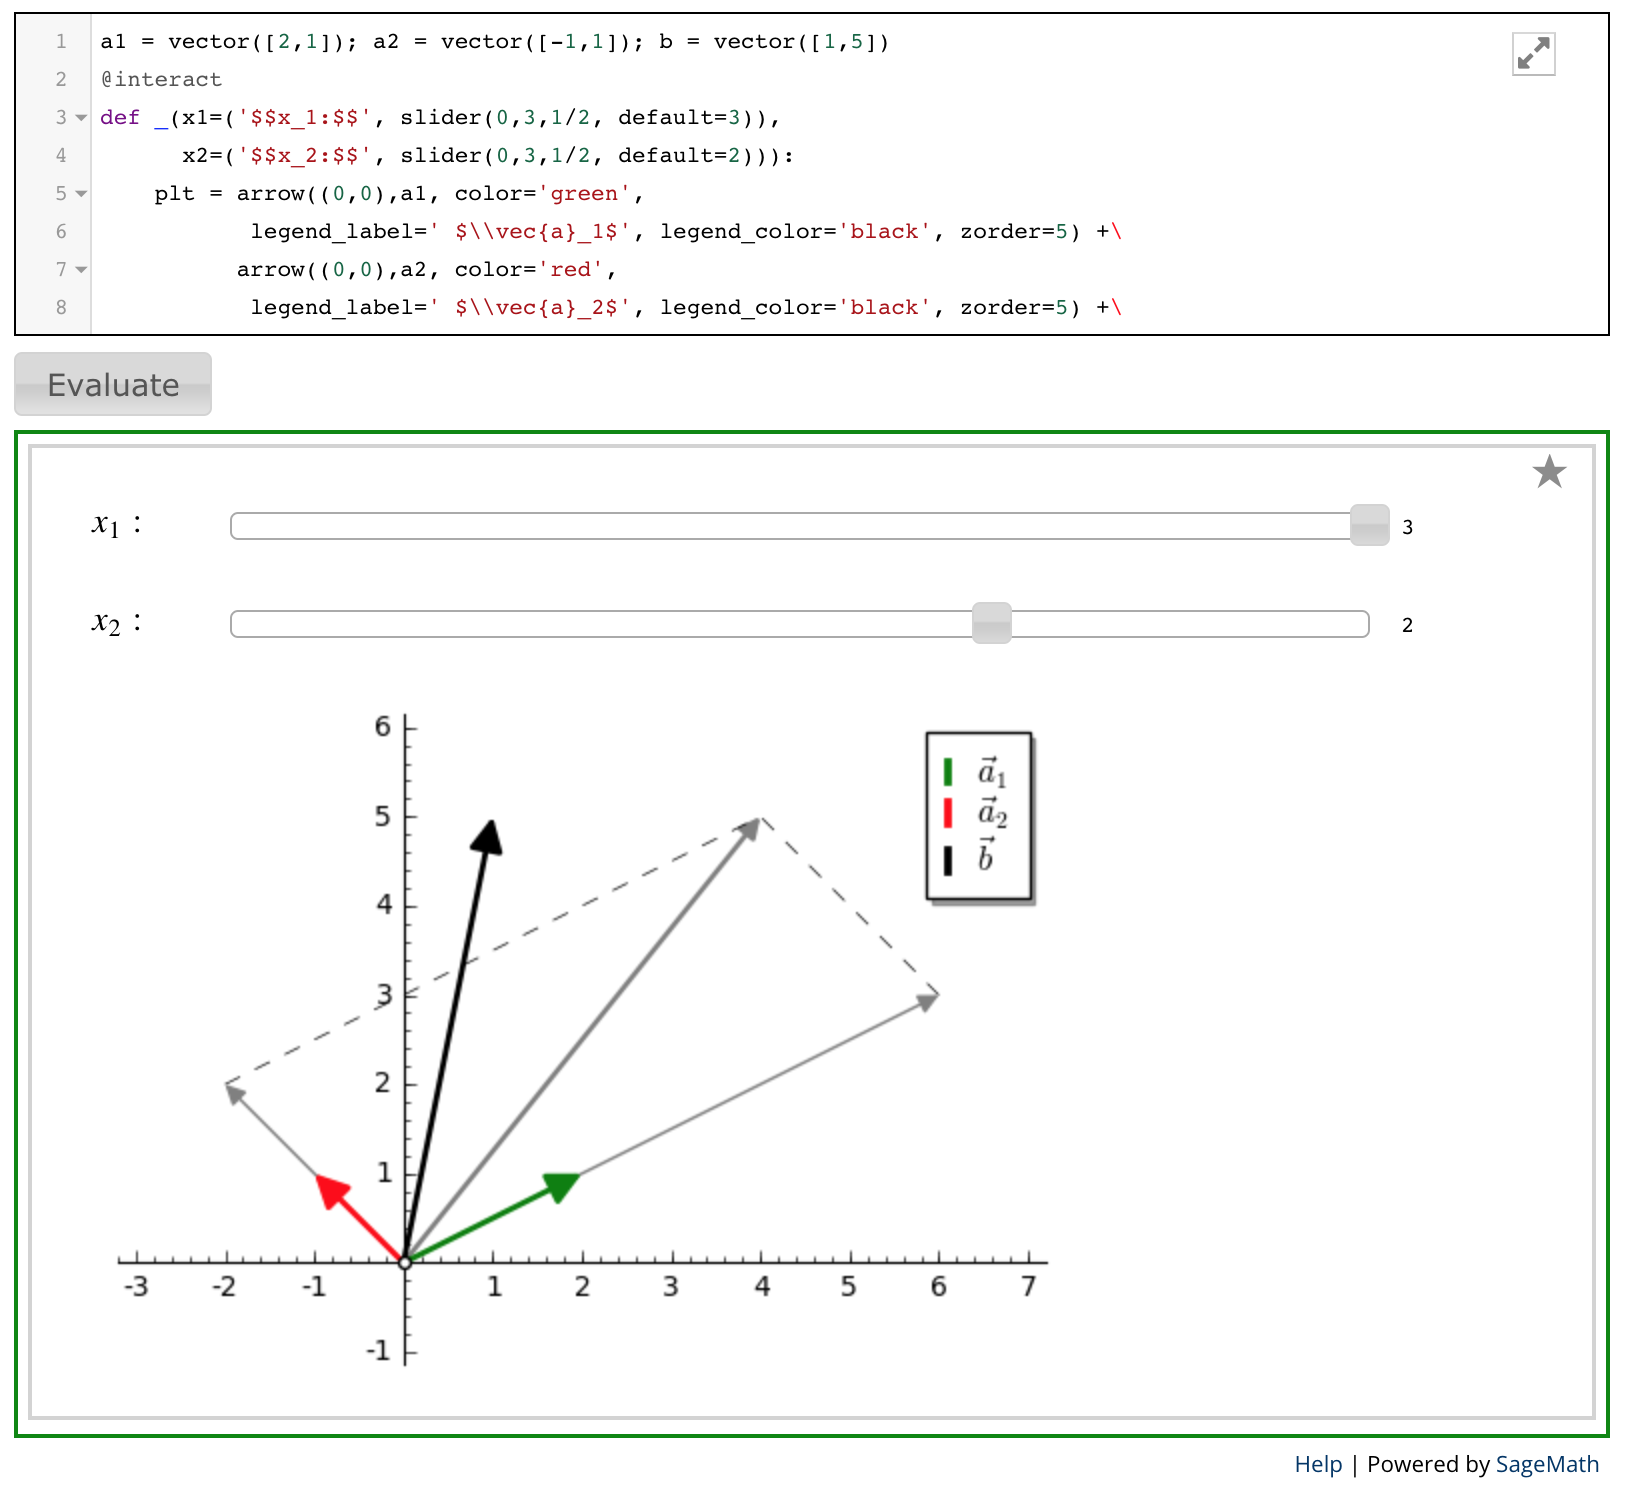
\includegraphics[width=.7\textwidth]{interact_in_sphinx.png}}
\caption{\label{fig:interact_sphinx} An example of \texttt{@interact} in
  \Sphinx generated web version of interactive book. The upper box
  shows the code and the lower box shows the output.}
\end{figure}

\TODO{screenshots of the cover / title / table of contents pages of the book?}

\TODO{screenshots of some page of the book which includes one or
  several interactive chunks?}

\TODO{RST source code of that page}

\TODO{Some assessment of the ease of use of the whole authoring
  environment by teachers?}

\TODO{Quality control: are you using regression tests for the
  interactive examples? E.g. nbval, or sage-style tests like in the
  Sage documentation? for the book Computational Mathematics with
  Sage, we included the examples directly as doctests in the Sage
  source code, so that if a change in Sage breaks them we are
  immediately aware of it, even before it get merged into master. Of
  course, for interacts, automatic testing is harder; maybe comment on
  strategies to test and avoid regressions you may have; e.g. having
  many readers and encouraging feedback.}

\TODO{Encouraging contributions: ``edit this page'' that points to the
  sources on github, with PR's and continous integration? See also our
  D3.5 deliverable
  https://github.com/OpenDreamKit/OpenDreamKit/issues/64 that enables
  this for the Sage documentation, and
  https://more-sagemath-tutorials.readthedocs.io/
  Would it make sense to host the books on ReadTheDocs?
}

\section{ Nonlinear Processes in Biology }


The book is in large extend based on coursework taught at University
of Silesia. It was primarily based on sagenb system and gradually was
converted into the interactive book with live examples.


The book covers the classical topics in modeling in
biology. Methodologically it can be split into the following topics:

\begin{enumerate}
\item Methods of mathematical modelling of  processes based on ODE and PDE. 
\item Qualitative methods in ODE and PDE with application of Sage. It
  includes:
  \begin{itemize}
  \item stationary states of the system,
  \item the linear stability of fix points,
  \item phase curves,
  \item bifurcation diagrams,
  \item time-dependent solutions,
  \item a graphical  presentation of all above  elements. 
  \end{itemize}
  
  For each subject there is a list of related problems and
  supplementary tasks as homework. All requires symbolic manipulations
  as well as certain techniques from numerical analysis like root
  finding.
  
\item Numerical solving of ODEs. It is complementary to analytical and
  qualitative methods for ODE. 
\item Numerical solving of PDE-s - diffusion equation,
  reaction-diffusion systems and similar. It requires good tools in data
  processing, usually uses numpy for calculations.

\end{enumerate}


It turned out that conceptually simple methods - like plotting a
function of one variable, which depends on a parameter (see
Figure.~\ref{fig:interact2}), can be very useful for the analysis of
models containing analytically untractable expressions. In this
particular example, students construct just a simple plot of a
function; then, with the help of \texttt{@interact} construction, the
plot is easily turned intro an applet for the analysis of the system.

The book covers the following  models: 
 \begin{itemize}
  \item one-dimensional systems (Malthus, Verhulst, Ludwig, Alee models);
  \item two-dimensional systems (Lotka-Volterra, May models);
  \item kinetics of chemical reactions;
  \item Belousov-Zhabotinsky reactions;
  \item models of epidemics.
 \end{itemize}

\begin{figure}
\centerline{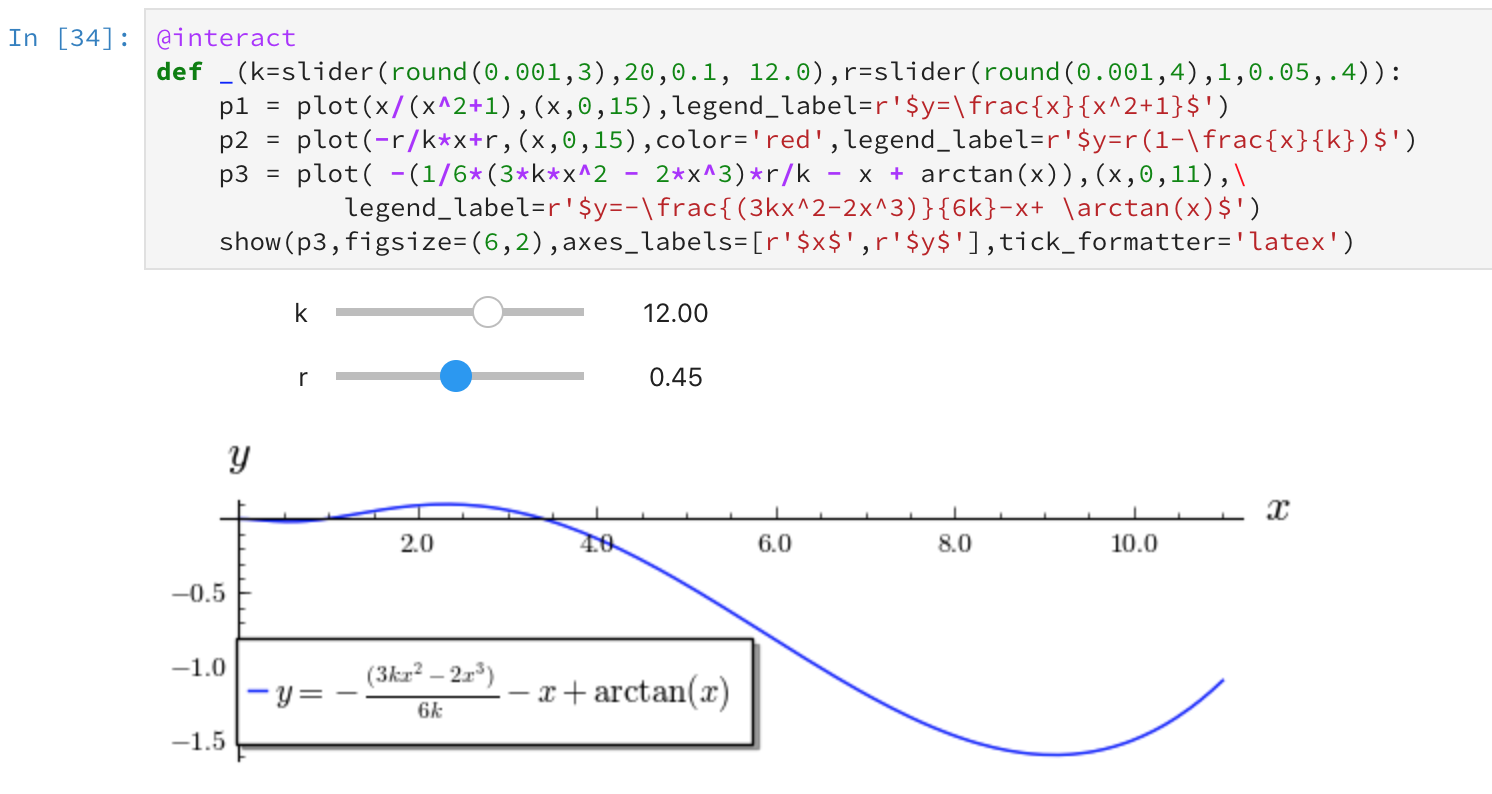
\includegraphics[width=.7\textwidth]{interact_npb.png}}
\caption{\label{fig:interact2} An example of \texttt{@interact}
  applied for graphical examination of roots of a function. It is a
  first step in qualitative analysis of model of tumor growth in a
  book.  }
\end{figure}



\section{Lectures on Linear Algebra}

This book is based on Linear Algebra courses for physics students
taught in recent years at the University of Silesia. It has been
gradually equipped with interactive materials and extended by sections
illustrating application of linear algebra in economy, computer
science, and other areas. The computations and the interactive part are
performed by \Sage, which is embedded in the book.

Along the theory the user becomes familiar with the code used in
\Sage. Their learning process is enhanced by various factors:
\begin{itemize}
\item numerous visualisations;
\item interactive images which allows for the construction of a
  graphical solution to a problem; the problem may be changed in real
  time by the user changing the code;
\item a place for experiments: the user may fill in the gaps in the code
  to produce graphical interpretation of a chosen operation;
\item possibility to perform the calculations with \Sage within the
  book; in particular, computations with real data and, thus, real
  life conclusions are possible;
\item some longer coding exercises are equipped with check points
  (without revealing the answer) to ensure that the discovered
  solution is correct.
\end{itemize}

Moreover, not only users benefit from interactive resources, but also
learn how to produce them themselves.

\section{Future work}

\TODO{Comments about language issues? Are the book written in both
  Polish and English? If so, how do you keep the two versions in
  sync? How time consuming is that process?}

The two open textbooks are put to continuous use for the eponymous
courses at university of Silesia; they are frequently updated with new
material (new models, exercises, ...), and improved according to
feedback from teachers and students. Also there are effort being done
to encourage other lecturers to use them and contribute back.

\end{document}

%%% Local Variables:
%%% mode: latex
%%% TeX-master: t
%%% End:

